% Standalone preview compile of every figure and table planned for the thesis.
% Compile with:  xelatex preview_all_figures.tex
% Output:        preview_all_figures.pdf  (one PDF page per figure/table, with
%                                          thesis-style caption + label + xref
%                                          example, at the same 12pt body and
%                                          1.5 line spacing the thesis uses).
%
% Purpose: lets us visually inspect how each figure looks at thesis text width
% with its caption, *without* touching the chapter source files. Mohammed's
% Track A edits happen in chapter*.tex; this file is read-only sandbox.
%
% Paths resolve via \graphicspath to output/pdf/.

\documentclass[12pt,a4paper]{report}
\usepackage{fontspec}
\usepackage{geometry}
\geometry{margin=1in}
\usepackage{setspace}
\setstretch{1.5}
\setlength{\parindent}{0pt}
\setlength{\parskip}{0.5em}
\usepackage{graphicx}
\usepackage{caption}
\usepackage{float}
\usepackage{booktabs}
\usepackage{xcolor}
\usepackage{enumitem}
\usepackage{hyperref}
\graphicspath{{output/pdf/}{system_diagrams/}}

% Helper: page header for each figure showing what we're previewing
\newcommand{\previewheader}[3]{%
  \vspace*{-2em}%
  \noindent\colorbox{black!8}{\parbox{\linewidth}{\vspace{2pt}%
    \textbf{\large #1} \quad \textit{#2}\\[2pt]%
    \textcolor{gray}{Planned section: #3}%
  \vspace{2pt}}}\\[1em]%
}

\title{Thesis Figures — Standalone Preview}
\author{Generated by \texttt{thesis\_figures/preview\_all\_figures.tex}}
\date{Compile to inspect every figure + table at thesis text width and caption style.}

\begin{document}
\maketitle

\noindent This document is a visual preview of every figure and table planned
for the thesis, rendered with the same body font and line-spacing settings as
\texttt{1-main.tex}. Each entry shows: (1) the figure or table, (2) the caption
exactly as it would appear under \texttt{\textbackslash caption}, (3) the
\texttt{\textbackslash label} used for cross-referencing, and (4) one example
in-body sentence that cites the figure.

\textbf{This is not the thesis itself.} Mohammed's Track A edits happen in
\texttt{Chapters/chapter*.tex}; this preview is a sandbox to confirm the
visual look before / during embedding.

\tableofcontents

% ════════════════════════════════════════════════════════════════════
\chapter{Chapter 2 — Literature Review \& Background}

% ─────────────────────────────────────────────────────────────────────
\previewheader{Figure 2.1}{RAG system architecture}{§2.1}
\begin{figure}[H]
  \centering
  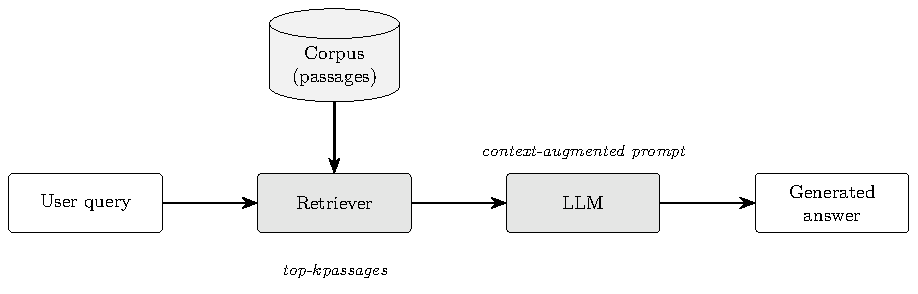
\includegraphics[width=0.85\textwidth]{fig_2_1_rag_arch.pdf}
  \caption{High-level architecture of a Retrieval-Augmented Generation (RAG) system. A user query is sent to a retriever that consults the corpus and returns the top-$k$ passages, which are passed alongside the query to an LLM to produce a context-augmented answer.}
  \label{fig:rag_arch}
\end{figure}
\textit{Example in-body cross-reference:}\\
``The Retrieval-Augmented Generation framework (Figure~\ref{fig:rag_arch}) couples a retriever with a generator, with the query enhancement layer of this thesis sitting between the user query and the retriever.''

% ─────────────────────────────────────────────────────────────────────
\newpage
\previewheader{Table 2.1}{Reviewed query-enhancement papers (13 entries)}{§2.4}
\begin{table}[H]
  \centering
  \caption{Query-enhancement papers reviewed for this thesis, with method family, evaluation dataset, and headline result.}
  \label{tab:reviewed_qe}
  \scriptsize
  \begin{tabular}{@{}>{\raggedright\arraybackslash}p{2.9cm}c>{\raggedright\arraybackslash}p{3.7cm}>{\raggedright\arraybackslash}p{2.4cm}>{\raggedright\arraybackslash}p{3.7cm}@{}}
\toprule
Paper & Year & Method & Dataset & Key result \\
\midrule
Query2Doc (Wang et al.) & 2023 & LLM pseudo-document concatenation & MS MARCO + BEIR & +8 NDCG@10 on MS MARCO with GPT-3 \\
HyDE (Gao et al.) & 2022 & LLM hypothetical document & TREC-DL / BEIR & strong zero-shot improvements \\
GAR (Mao et al.) & 2021 & LLM generates answer/context for query rewriting & open-domain QA & competitive with supervised reranking \\
GRF (Mackie et al.) & 2023 & Generative Relevance Feedback for dense & TREC-DL & \textasciitilde +10 MAP; fusion best \\
CSQE (Lei et al.) & 2024 & Corpus-Steered Query2Doc & TREC-DL & +30\% MAP over BM25 \\
MuGI (Zhang et al.) & 2024 & Multi-Text Generation Integration & BEIR & best QE practices study \\
ThinkQE (Lei et al.) & 2025 & Iterative chain-of-thought expansion & TREC-DL & state of the art on multi-step queries \\
Exp4Fuse (Liu et al.) & 2025 & Original + expanded query via modified RRF & multiple & nearest prior art to thesis \\
DAPR (Wang et al.) & 2024 & Dense Approach via Pre-trained Retrievers & academic IR & context-rich expansion \\
AQE (Yang et al.) & 2025 & Aligned Query Expansion via LLM alignment & academic IR & efficient at scale \\
KAR (Xia et al.) & 2025 & Knowledge-Aware Query Expansion & textual + relational retrieval & strong on relational \\
Song \& Zheng (survey) & 2024 & Query optimisation taxonomy (4 operations) & --- & defines expansion, decomposition, disambiguation, abstraction \\
QE survey (arXiv 2509.07794) & 2025 & Comprehensive QE survey in the LLM era & --- & recent QE families \\
\bottomrule
\end{tabular}

\end{table}
\textit{Example in-body cross-reference:}\\
``Table~\ref{tab:reviewed_qe} summarises the query-enhancement literature, grouped by whether the technique is lexical (PRF, RM3, BM25 expansion) or LLM-based generative (Query2Doc, HyDE, CSQE, MuGI, ThinkQE, Exp4Fuse).''

% ─────────────────────────────────────────────────────────────────────
\newpage
\previewheader{Table 2.2}{LLM models used in this thesis (11 entries)}{§2.5}
\begin{table}[H]
  \centering
  \caption{Open-source LLMs evaluated for Arabic query enhancement, ordered by parameter count.}
  \label{tab:models_used}
  \scriptsize
  \begin{tabular}{llcccc}
\toprule
Model & Family & Params (B) & Multilingual & Arabic-specialised & Quantisation \\
\midrule
SILMA Kashif-2B & Silma AI & 2 & No & Yes (RAG) & FP16 \\
Qwen 2.5 3B & Alibaba & 3 & Yes (29 langs) & No & FP16 \\
Falcon-H1-3B & TII & 3 & Yes & Yes & BF16 \\
Qwen3-4B & Alibaba & 4 & Yes (119 langs) & No & FP16 \\
Gemma 3 4B & Google & 4 & Yes & No & FP16/BF16 \\
Qwen 2.5-7B & Alibaba & 7 & Yes (29 langs) & No & FP16 \\
ALLaM-7B (DROPPED) & NCAI & 7 & Yes & Yes & FP16 \\
Jais-2-8B & G42 & 8 & Yes & Yes & BF16 \\
Qwen3-8B & Alibaba & 8 & Yes (119 langs) & No & FP16 \\
Aya Expanse 8B & Cohere & 8 & Yes (101 langs) & No & 4-bit NF4 \\
\bottomrule
\end{tabular}

\end{table}
\textit{Example in-body cross-reference:}\\
``The eleven models in Table~\ref{tab:models_used} span 2 B--20 B parameters, with both multilingual generalists (Qwen 2.5, Qwen3, Gemma 3, Aya Expanse) and Arabic-specialised models (SILMA Kashif, Falcon-H1, Jais-2, ALLaM).''

% ════════════════════════════════════════════════════════════════════
\chapter{Chapter 3 — Methodology}

% ─────────────────────────────────────────────────────────────────────
\previewheader{Figure 3.1}{End-to-end thesis pipeline}{§3.1}
\begin{figure}[H]
  \centering
  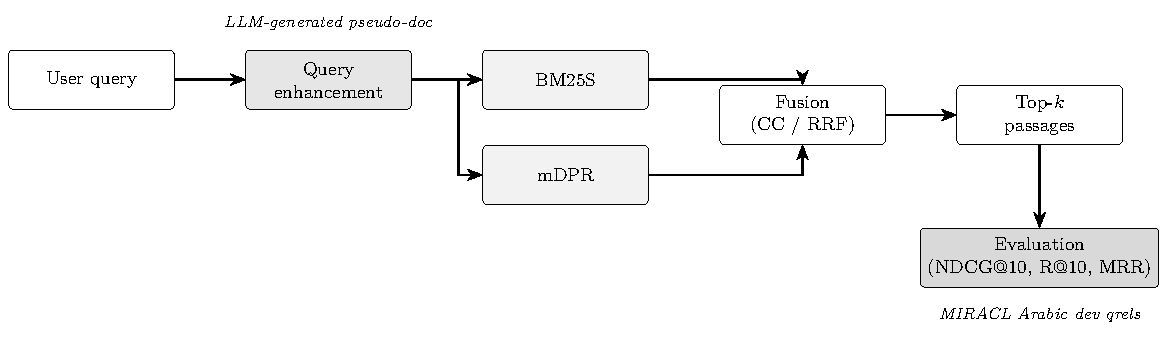
\includegraphics[width=0.95\textwidth]{fig_3_1_pipeline.pdf}
  \caption{The thesis evaluation pipeline. A user query passes through the query-enhancement layer, after which BM25S and mDPR retrieve independently; their ranked lists are then fused (CC or RRF) and the top-$k$ passages are scored against the MIRACL Arabic dev qrels.}
  \label{fig:pipeline}
\end{figure}
\textit{Example in-body cross-reference:}\\
``Figure~\ref{fig:pipeline} shows the overall evaluation pipeline used throughout this thesis; subsequent sections describe each stage in detail.''

% ─────────────────────────────────────────────────────────────────────
\newpage
\previewheader{Figure 3.3}{BM25S indexing flow}{§3.4}
\begin{figure}[H]
  \centering
  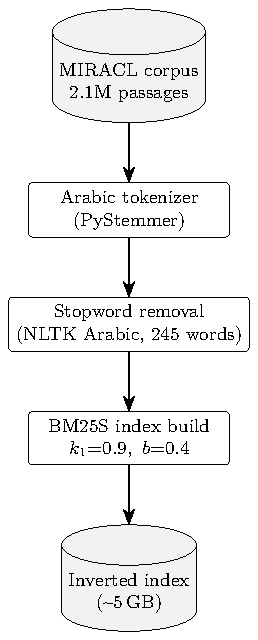
\includegraphics[width=0.65\textwidth]{fig_3_3_bm25s.pdf}
  \caption{BM25S indexing pipeline applied to the MIRACL Arabic corpus. Passages are tokenised with PyStemmer, stopword-removed using 245 Arabic stopwords, then indexed under BM25S with $k_1{=}0.9$ and $b{=}0.4$.}
  \label{fig:bm25s_indexing}
\end{figure}
\textit{Example in-body cross-reference:}\\
``The sparse retrieval pipeline (Figure~\ref{fig:bm25s_indexing}) uses BM25S, a pure-Python BM25 implementation, with Arabic-aware tokenisation and stopword removal.''

% ─────────────────────────────────────────────────────────────────────
\newpage
\previewheader{Figure 3.4}{mDPR encoding flow}{§3.5}
\begin{figure}[H]
  \centering
  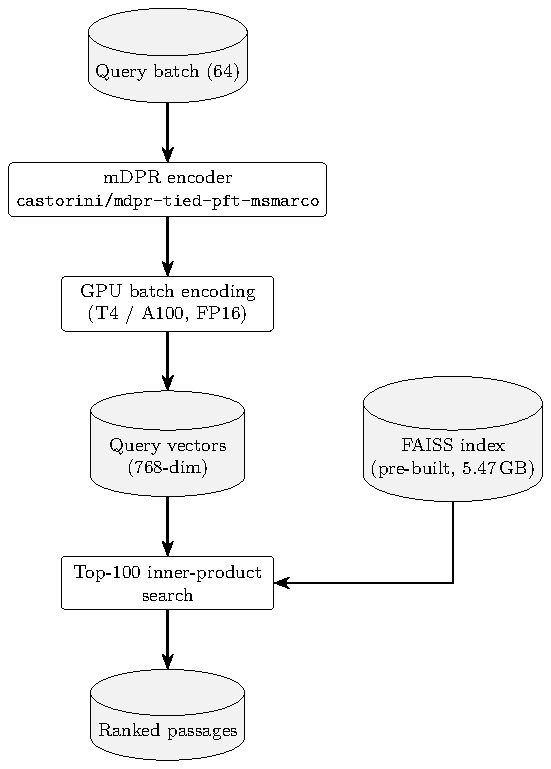
\includegraphics[width=0.7\textwidth]{fig_3_4_mdpr.pdf}
  \caption{Dense retrieval pipeline using multilingual DPR. Queries are encoded in batches on a single A100 GPU under FP16; the resulting 768-dimensional vectors are searched against a pre-built FAISS index of the corpus.}
  \label{fig:mdpr_encoding}
\end{figure}
\textit{Example in-body cross-reference:}\\
``Dense retrieval (Figure~\ref{fig:mdpr_encoding}) is implemented via the multilingual DPR encoder \texttt{castorini/mdpr-tied-pft-msmarco}, applied to the pre-built MIRACL FAISS index.''

% ─────────────────────────────────────────────────────────────────────
\newpage
\previewheader{Figure 3.5}{Query2Doc generation}{§3.6}
\begin{figure}[H]
  \centering
  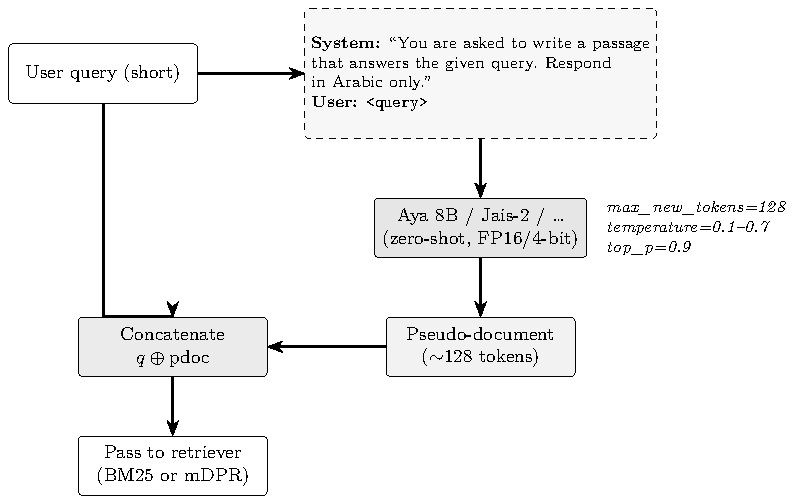
\includegraphics[width=0.95\textwidth]{fig_3_5_query2doc.pdf}
  \caption{Query2Doc generation: the original query is wrapped in a fixed prompt template, an open-source LLM generates a short pseudo-document conditioned on the query, and the pseudo-document is concatenated with the query before being passed to the retriever.}
  \label{fig:query2doc}
\end{figure}
\textit{Example in-body cross-reference:}\\
``The Query2Doc pipeline (Figure~\ref{fig:query2doc}) follows the original Wang et al. (2023) formulation, with the LLM and generation parameters varied per experiment.''

% ─────────────────────────────────────────────────────────────────────
\newpage
\previewheader{Figure 3.7}{Hybrid fusion (Convex Combination and RRF)}{§3.7}
\begin{figure}[H]
  \centering
  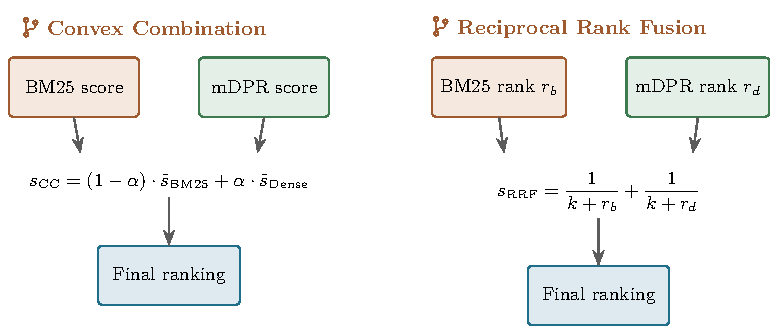
\includegraphics[width=0.95\textwidth]{fig_3_7_hybrid.pdf}
  \caption{Two retriever-fusion methods evaluated in this thesis. Convex Combination (left) computes a weighted sum of normalised retrieval scores; Reciprocal Rank Fusion (right) sums the reciprocal of each retriever's rank for every document.}
  \label{fig:hybrid_fusion}
\end{figure}
\textit{Example in-body cross-reference:}\\
``Two complementary fusion strategies (Figure~\ref{fig:hybrid_fusion}) are evaluated: CC requires score normalisation, while RRF is parameter-light and operates on ranks alone.''

% ─────────────────────────────────────────────────────────────────────
\newpage
\previewheader{Figure 3.8}{CSQE pipeline (three-stage)}{§3.8}
\begin{figure}[H]
  \centering
  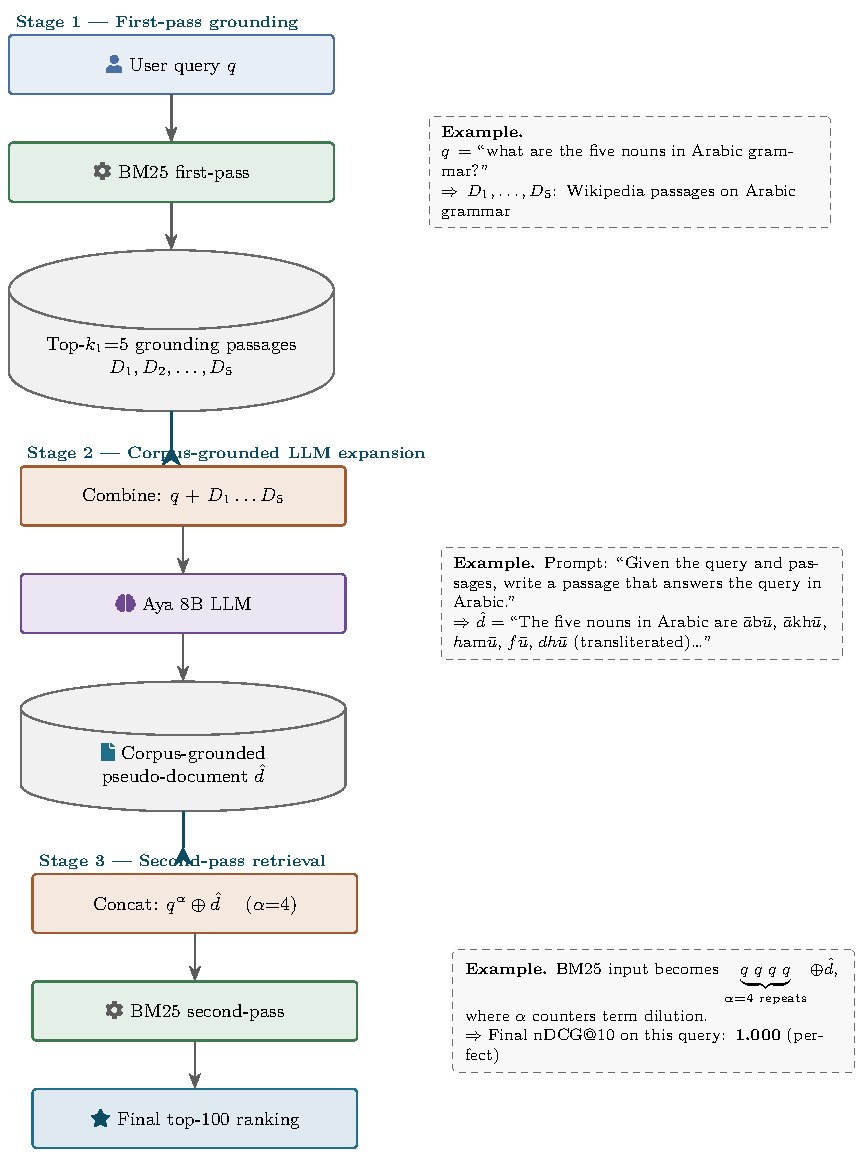
\includegraphics[width=0.95\textwidth]{fig_3_8_csqe.pdf}
  \caption{Corpus-Steered Query Expansion (CSQE) pipeline. Stage 1: BM25 retrieves a first-pass top-$k_1$ context. Stage 2: corpus context plus the original query are fed to the Aya LLM, which generates a corpus-grounded pseudo-document. Stage 3: the query (repeated $\alpha$ times) is concatenated with the pseudo-document and fed to a BM25 second pass.}
  \label{fig:csqe_pipeline}
\end{figure}
\textit{Example in-body cross-reference:}\\
``The corpus-steered variant (Figure~\ref{fig:csqe_pipeline}) replaces the blind LLM expansion of Figure~\ref{fig:query2doc} with one grounded in the corpus, mitigating the entity-hallucination failures observed in the blind setting.''

% ─────────────────────────────────────────────────────────────────────
\newpage
\previewheader{Figure 3.9}{Best system architecture (BM25-only-expanded RRF $k=20$)}{§3.8.3 / §4.7}
\begin{figure}[H]
  \centering
  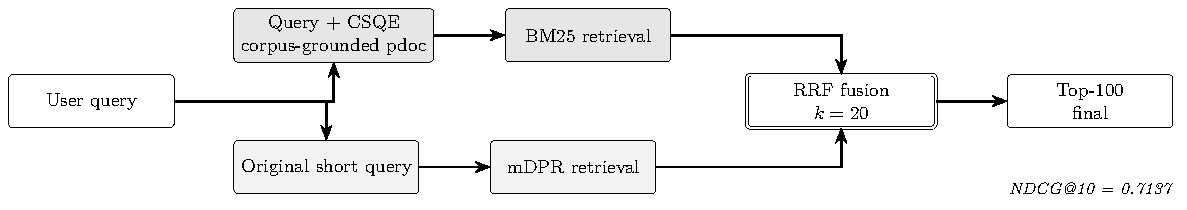
\includegraphics[width=0.95\textwidth]{fig_3_9_best_system.pdf}
  \caption{Architecture of the thesis's best-performing system. CSQE-expanded queries are fed to BM25 while the original short queries are fed to mDPR; the two ranked lists are fused with Reciprocal Rank Fusion ($k=20$), yielding the headline nDCG@10 of 0.714.}
  \label{fig:best_system}
\end{figure}
\textit{Example in-body cross-reference:}\\
``The best-performing configuration (Figure~\ref{fig:best_system}) applies expansion asymmetrically: only the sparse retriever receives the CSQE-grounded query.''

% ─────────────────────────────────────────────────────────────────────
\newpage
\previewheader{Table 3.1}{Per-model hardware configuration (9 rows)}{§3.6}
\begin{table}[H]
  \centering
  \caption{Hardware and precision configuration used for each LLM evaluated, plus the per-model batch size and total wall-clock runtime on the MIRACL dev set.}
  \label{tab:hardware_config}
  \scriptsize
  \begin{tabular}{llllll}
\toprule
Model & GPU & Precision & Batch & Runtime (min) & Notes \\
\midrule
SILMA Kashif-2B & A100 40GB & FP16 & 16 & 15--20 & -- \\
Qwen 2.5 3B & A100 40GB & FP16 & 8 & \textasciitilde 40 & -- \\
Falcon-H1-3B & A100 40GB & BF16 & 1 & \textasciitilde 60 & hybrid Mamba; batching broken \\
Qwen3-4B & A100 40GB & FP16 & 32 & \textasciitilde 25 & enable\_thinking=False \\
Gemma 3 4B & A100 40GB & FP16/BF16 & 16 & \textasciitilde 30 & numerical-stability fixes (BF16) \\
Qwen 2.5-7B & A100 40GB & FP16 & 16 & \textasciitilde 35 & -- \\
Jais-2-8B & A100 40GB & BF16 & 8 & \textasciitilde 50 & token\_type\_ids removed; BF16 mandatory (Squared-ReLU overflow in FP16) \\
Qwen3-8B & A100 40GB & FP16 & 16 & \textasciitilde 40 & thinking tags stripped \\
Aya Expanse 8B & A100 40GB & 4-bit NF4 & 8 & \textasciitilde 50 & -- \\
\bottomrule
\end{tabular}

\end{table}
\textit{Example in-body cross-reference:}\\
``All experiments ran on a single A100 40 GB GPU under the configurations listed in Table~\ref{tab:hardware_config}.''

% ─────────────────────────────────────────────────────────────────────
\newpage
\previewheader{Table 3.2}{Per-model generation hyperparameters (9 rows)}{§3.6}
\begin{table}[H]
  \centering
  \caption{Pseudo-document generation hyperparameters per model. Temperature, top-$p$ and max\_new\_tokens were tuned per model where the model card specified recommended values; default otherwise.}
  \label{tab:gen_hyperparams}
  \scriptsize
  \begin{tabular}{lllll}
\toprule
model & temperature & top_p & max_new_tokens & special \\
\midrule
SILMA Kashif-2B & 0.1000 & 0.9000 & 128 & temp 0.1 chosen empirically over 0.7 (+2.5%) \\
Qwen 2.5 3B & 0.7000 & 0.9000 & 128 & original Query2Doc default \\
Falcon-H1-3B & 0.1000 & 0.9000 & 128 & model-recommended (>0.1 drops performance) \\
Qwen3-4B & 0.7000 & 0.9000 & 128 & enable_thinking=False; do_sample=True (greedy gives infinite repetitions) \\
Gemma 3 4B & 0.1000 & 0.9000 & 128 & -- \\
Qwen 2.5-7B & 0.1000 & 0.9000 & 128 & -- \\
Jais-2-8B & 0.7000 & 0.9000 & 128 & token_type_ids not passed \\
Qwen3-8B & 0.1000 & 0.9000 & 128 & thinking tags stripped at decode time \\
Aya Expanse 8B & 0.1000 & 0.9000 & 128 & -- \\
\bottomrule
\end{tabular}

\end{table}
\textit{Example in-body cross-reference:}\\
``Generation hyperparameters per model are summarised in Table~\ref{tab:gen_hyperparams}; the largest model-specific deviations were Falcon-H1's recommended temperature of 0.1 and Qwen3's mandatory \texttt{enable\_thinking=False}.''

% ════════════════════════════════════════════════════════════════════
\chapter{Chapter 4 — Results \& Discussion}

% ─────────────────────────────────────────────────────────────────────
\previewheader{Table 4.1}{Baselines: mDPR vs BM25}{§4.1}
\begin{table}[H]
  \centering
  \caption{Baseline retrieval performance on the MIRACL Arabic dev set (2,896 queries). All metrics rounded to three decimals.}
  \label{tab:baselines}
  \begin{tabular}{lcccc}
\toprule
Retriever & Recall@10 & Recall@100 & NDCG@10 & MRR \\
\midrule
mDPR (Dense) & 0.616 & 0.841 & NaN & NaN \\
BM25S (Sparse) & 0.596 & 0.858 & NaN & NaN \\
\bottomrule
\end{tabular}

\end{table}
\textit{Example in-body cross-reference:}\\
``As Table~\ref{tab:baselines} shows, mDPR and BM25 are complementary: BM25 has higher recall at 100 but lower precision in the top 10.''

% ─────────────────────────────────────────────────────────────────────
\newpage
\previewheader{Figure 4.1}{Per-query nDCG@10 distribution (mDPR vs BM25)}{§4.1}
\begin{figure}[H]
  \centering
  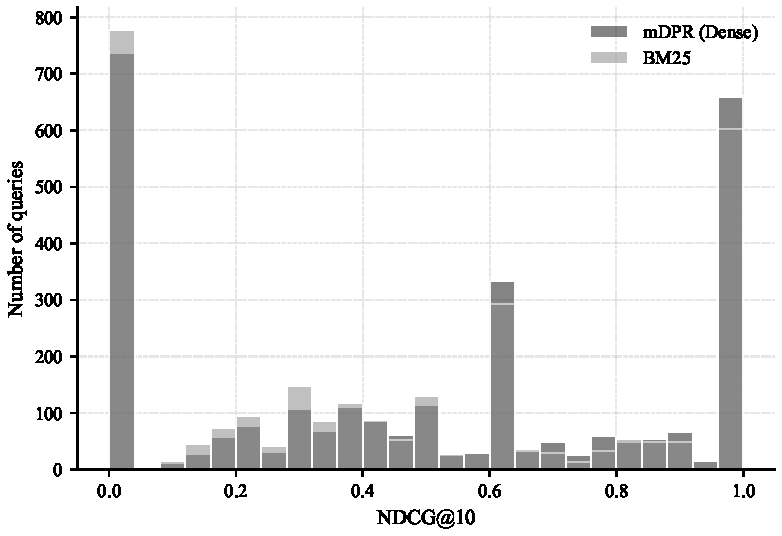
\includegraphics[width=0.85\textwidth]{fig_4_1_ndcg_hist_v1.pdf}
  \caption{Per-query nDCG@10 distribution for the two baseline retrievers on the MIRACL Arabic dev set. Both retrievers exhibit a bimodal distribution: a large mass of queries near zero (poorly served) and another mass near one (perfectly served), with relatively few in the middle range.}
  \label{fig:per_query_dist}
\end{figure}

% ─────────────────────────────────────────────────────────────────────
\newpage
\previewheader{Figure 4.2}{Failure cliff — 33.9\% of queries score nDCG@10 $<$ 0.3}{§4.2.1}
\begin{figure}[H]
  \centering
  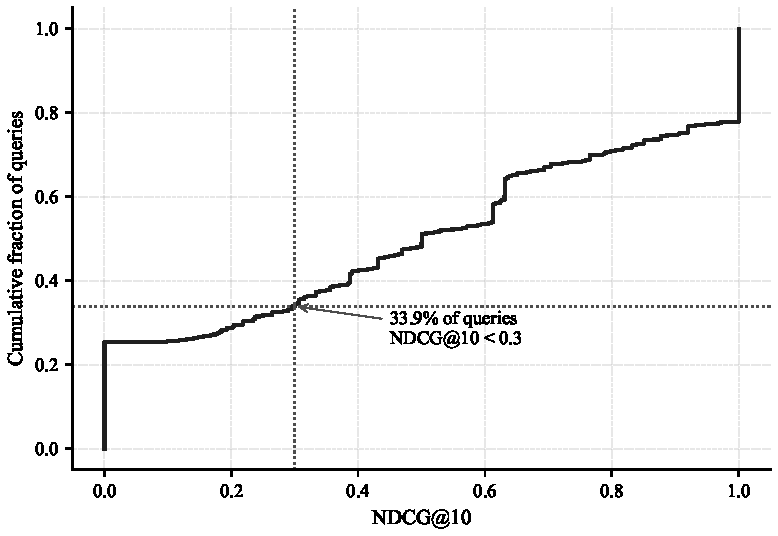
\includegraphics[width=0.85\textwidth]{fig_4_2_failure_cliff_v1.pdf}
  \caption{Cumulative distribution of per-query nDCG@10 on the mDPR baseline. The marked threshold at 0.3 separates 33.9\% of queries on which the baseline performs poorly from the remainder.}
  \label{fig:failure_cliff}
\end{figure}

% ─────────────────────────────────────────────────────────────────────
\newpage
\previewheader{Figure 4.3}{nDCG@10 by query length (1--3 / 4--8 / 9+ words) — \textbf{v2 violin}}{§4.2.2}
\begin{figure}[H]
  \centering
  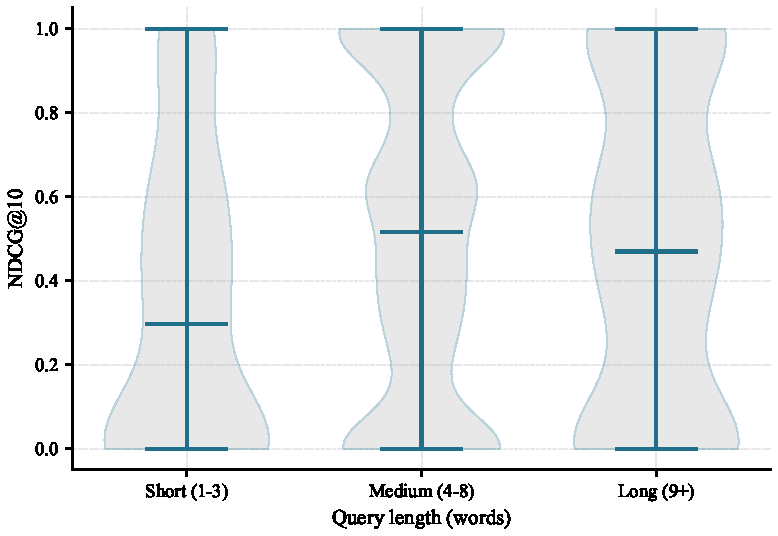
\includegraphics[width=0.85\textwidth]{fig_4_3_length_violin_v2.pdf}
  \caption{Distribution of mDPR nDCG@10 within each query-length bucket. Short queries (1--3 words) achieve the lowest mean nDCG@10 (0.345) while medium queries (4--8 words) achieve the highest (0.511); the relationship is non-monotonic, not a linear trend.}
  \label{fig:length_dist}
\end{figure}

% ─────────────────────────────────────────────────────────────────────
\newpage
\previewheader{Figure 4.4}{Recall@$k$ curve, $k = 1\ldots 100$}{§4.2.3}
\begin{figure}[H]
  \centering
  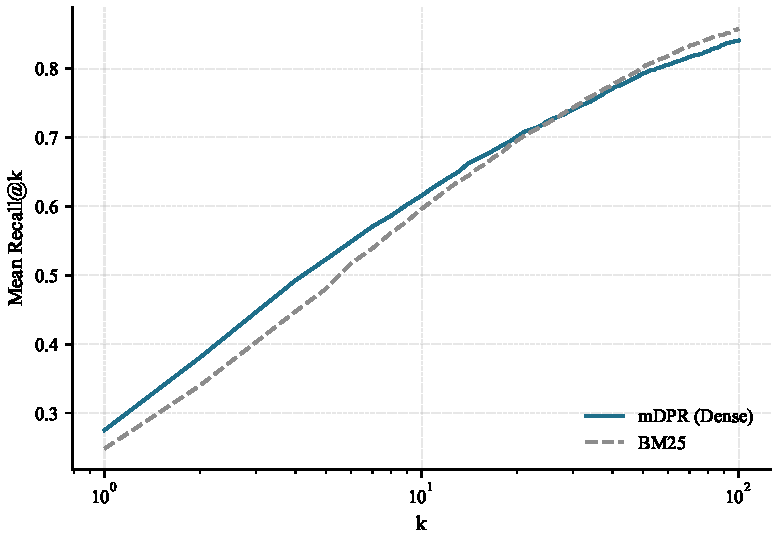
\includegraphics[width=0.85\textwidth]{fig_4_4_recall_curve.pdf}
  \caption{Mean Recall@$k$ for mDPR and BM25 on the MIRACL Arabic dev set, $k$ on a log axis. Approximately 10\% of relevant passages remain unrecovered even at depth 100, motivating hybrid retrieval and corpus-steered expansion.}
  \label{fig:recall_curve}
\end{figure}

% ─────────────────────────────────────────────────────────────────────
\newpage
\previewheader{Table 4.2}{Dense-retrieval results across 10 LLMs}{§4.3}
\begin{table}[H]
  \centering
  \caption{Query2Doc dense-retrieval results across ten LLMs, ordered by nDCG@10. Aya Expanse 8B leads at 0.616.}
  \label{tab:dense_models}
  \scriptsize
  \begin{tabular}{lccccccl}
\toprule
model & params_B & ndcg_10 & recall_10 & recall_100 & mrr & delta & note \\
\midrule
Aya Expanse 8B & 8.0000 & 0.6164 & 0.7256 & 0.9001 & 0.6493 & 0.1171 & blind QE \\
Jais-2-8B & 8.0000 & 0.6018 & 0.7161 & 0.8981 & 0.6356 & 0.1025 & - \\
Qwen3-8B & 8.0000 & 0.5958 & - & - & - & 0.0965 & from CLAUDE.md kernel \\
Aya 8B CSQE & 8.0000 & 0.5915 & 0.7073 & 0.8816 & 0.6225 & 0.0922 & CSQE variant \\
Qwen 2.5-7B & 7.0000 & 0.5813 & - & - & - & 0.0820 & from CLAUDE.md kernel \\
Qwen3-4B & 4.0000 & 0.5691 & 0.6824 & 0.8726 & 0.6015 & 0.0698 & - \\
Qwen 2.5 3B & 3.0000 & 0.5435 & 0.6608 & 0.8594 & 0.5742 & 0.0442 & - \\
Gemma 3 4B & 4.0000 & 0.5435 & - & - & - & 0.0442 & from CLAUDE.md kernel \\
Falcon-H1-3B & 3.0000 & 0.5359 & 0.6484 & 0.8531 & 0.5681 & 0.0366 & - \\
SILMA Kashif-2B & 2.0000 & 0.5178 & - & - & - & 0.0185 & from CLAUDE.md kernel \\
mDPR (no QE) & - & 0.4993 & 0.6156 & 0.8407 & 0.5328 & 0.0000 & baseline \\
ALLaM-7B & 7.0000 & 0.2550 & 0.3335 & 0.5465 & 0.2708 & -0.2443 & DROPPED (tokenizer bug) \\
\bottomrule
\end{tabular}

\end{table}

% ─────────────────────────────────────────────────────────────────────
\newpage
\previewheader{Figure 4.5 v1}{Sorted nDCG@10 across 10 LLMs (vertical)}{§4.3 — also include v3 grouped per Osman}
\begin{figure}[H]
  \centering
  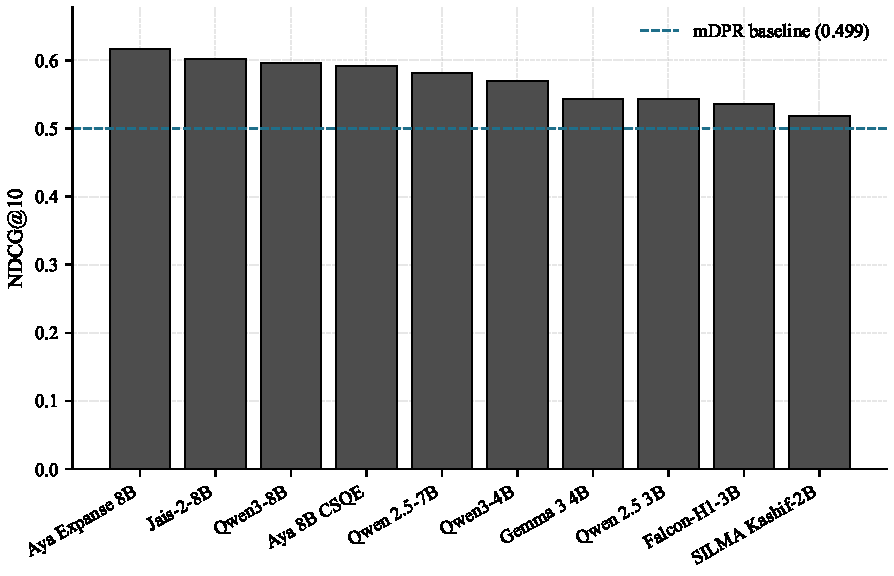
\includegraphics[width=0.95\textwidth]{fig_4_5_models_bar_v1.pdf}
  \caption{nDCG@10 of each evaluated LLM on the Query2Doc dense pipeline, sorted descending. The dashed reference line marks the mDPR baseline (0.499); each model uses its consistent thesis colour, identical to Figure~\ref{fig:repetition_sweep}.}
  \label{fig:models_bar}
\end{figure}

% ─────────────────────────────────────────────────────────────────────
\newpage
\previewheader{Figure 4.5 v3}{Multi-metric grouped variant}{§4.3 (companion to Fig 4.5)}
\begin{figure}[H]
  \centering
  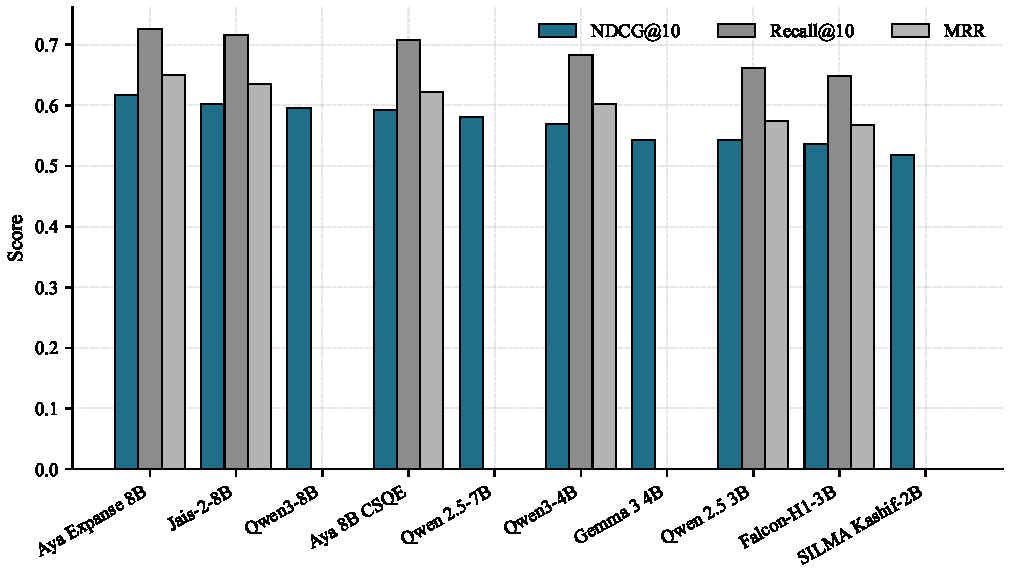
\includegraphics[width=0.95\textwidth]{fig_4_5_models_grouped_v3.pdf}
  \caption{Grouped per-model bars for nDCG@10, Recall@10 and MRR on the Query2Doc dense pipeline.}
  \label{fig:models_grouped}
\end{figure}

% ─────────────────────────────────────────────────────────────────────
\newpage
\previewheader{Figure 4.6 v2}{Model size vs $\Delta$ nDCG@10 (labelled + trendline)}{§4.3}
\begin{figure}[H]
  \centering
  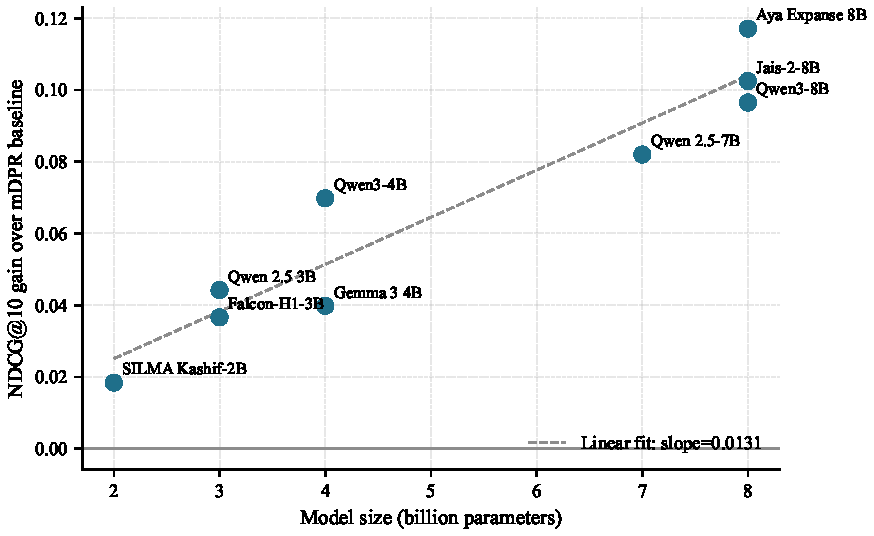
\includegraphics[width=0.85\textwidth]{fig_4_6_size_v2_labelled.pdf}
  \caption{Relationship between model parameter count (billions) and gain over the mDPR baseline. A weak positive trend is visible; the Qwen-family subset (3B--8B) corroborates the size-quality correlation within a single architecture.}
  \label{fig:size_vs_gain}
\end{figure}

% ─────────────────────────────────────────────────────────────────────
\newpage
\previewheader{Table 4.3}{Per-model BM25 best configurations (9 rows)}{§4.4 / §4.6}
\begin{table}[H]
  \centering
  \caption{Best BM25 query-repetition configuration per model. All nine models exceed the BM25 baseline (0.462) at their optimum repetition count.}
  \label{tab:bm25_best}
  \scriptsize
  \begin{tabular}{lrrrrrlrr}
\toprule
Model & Params (B) & $n{=}1$ nDCG@10 & $n{=}1$ R@10 & $n{=}1$ R@100 & $n{=}1$ MRR & Best config & Best nDCG@10 & $\Delta$ vs $n{=}1$ \\
\midrule
BM25 baseline (no QE) & -- & 0.4621 & 0.5964 & 0.8577 & 0.4836 & n=1 & 0.4621 & 0.0000 \\
SILMA 2B & 2.0000 & 0.4277 & 0.5550 & 0.8115 & 0.4485 & n=5 & 0.4832 & 0.0555 \\
Falcon-H1-3B & 3.0000 & 0.4038 & -- & -- & -- & n=10 & 0.5113 & 0.1075 \\
Qwen 2.5-3B & 3.0000 & 0.4090 & -- & -- & -- & n=5 & 0.5185 & 0.1095 \\
Qwen3-4B & 4.0000 & 0.4145 & -- & -- & -- & n=7 & 0.5244 & 0.1099 \\
Gemma 3 4B & 4.0000 & 0.3447 & 0.4532 & 0.7182 & 0.3718 & n=7 & 0.5277 & 0.1830 \\
Qwen 2.5-7B & 7.0000 & 0.4682 & 0.6040 & 0.8646 & 0.4905 & n=5 & 0.5358 & 0.0676 \\
Qwen3-8B & 8.0000 & 0.4459 & 0.5806 & 0.8499 & 0.4702 & n=7 & 0.5328 & 0.0869 \\
Jais-2-8B & 8.0000 & 0.5122 & -- & -- & -- & beta=2 & 0.5731 & 0.0609 \\
Aya Expanse 8B & 8.0000 & 0.5046 & 0.6284 & 0.8734 & 0.5377 & beta=2 & 0.5855 & 0.0809 \\
\bottomrule
\end{tabular}

\end{table}

% ─────────────────────────────────────────────────────────────────────
\newpage
\previewheader{Figure 4.7}{BM25 query-repetition sweep across 9 models}{§4.6}
\begin{figure}[H]
  \centering
  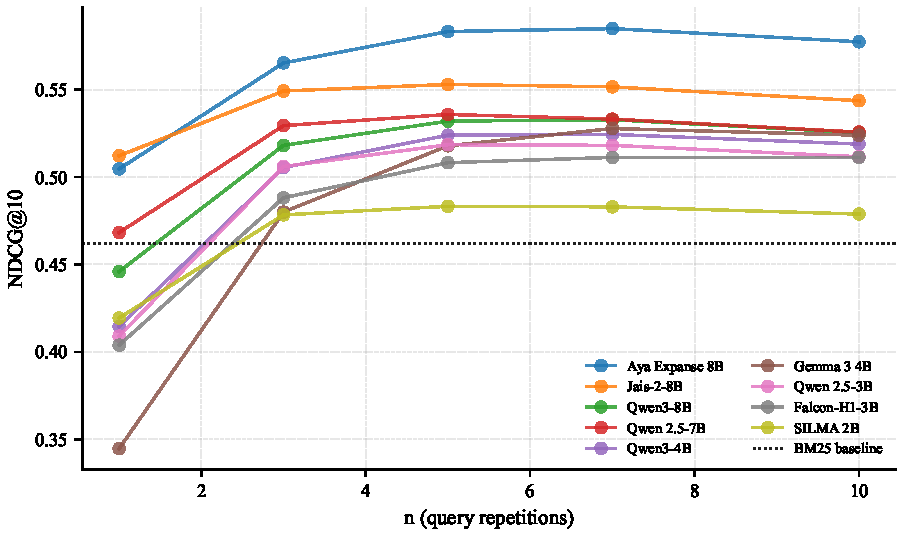
\includegraphics[width=0.95\textwidth]{fig_4_7_repetition_v1.pdf}
  \caption{nDCG@10 on the BM25 retriever as a function of query-repetition count $n$ for each LLM-generated pseudo-document. Six of nine models start below the BM25 baseline at $n{=}1$; all nine recover or exceed it at their optimum $n$. Colours match Figure~\ref{fig:models_bar}.}
  \label{fig:repetition_sweep}
\end{figure}

% ─────────────────────────────────────────────────────────────────────
\newpage
\previewheader{Figure 4.8}{Dense gain vs BM25 gain per model}{§4.4 / §4.6}
\begin{figure}[H]
  \centering
  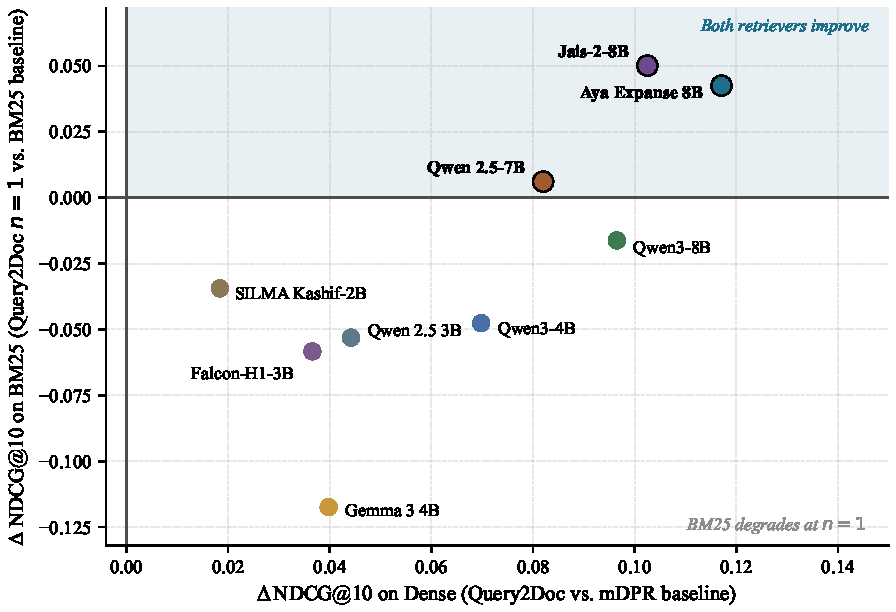
\includegraphics[width=0.85\textwidth]{fig_4_8_gains_v1.pdf}
  \caption{Per-model Query2Doc gain on the Dense retriever versus the BM25 retriever. Only Aya Expanse 8B and Jais-2 8B sit in the both-positive quadrant; most other models help Dense but degrade BM25 at $n{=}1$.}
  \label{fig:dense_vs_bm25_gains}
\end{figure}

% ─────────────────────────────────────────────────────────────────────
\newpage
\previewheader{Table 4.4}{Hybrid baselines (no QE)}{§4.7}
\begin{table}[H]
  \centering
  \caption{Hybrid retrieval baselines without query enhancement: BM25 alone, mDPR alone, and the two fusion variants.}
  \label{tab:hybrid_baselines}
  \begin{tabular}{lcccc}
\toprule
Method & nDCG@10 & Recall@10 & Recall@100 & MRR \\
\midrule
BM25 alone & 0.462 & 0.596 & 0.858 & 0.484 \\
mDPR alone & 0.499 & 0.616 & 0.841 & 0.533 \\
Hybrid CC (α=0.5) & 0.627 & 0.748 & 0.946 & 0.658 \\
Hybrid RRF (k=20) & 0.627 & 0.760 & 0.947 & 0.652 \\
\bottomrule
\end{tabular}

\end{table}

% ─────────────────────────────────────────────────────────────────────
\newpage
\previewheader{Figure 4.9 v2}{Hybrid CC $\alpha$ sweep — all four metrics}{§4.7}
\begin{figure}[H]
  \centering
  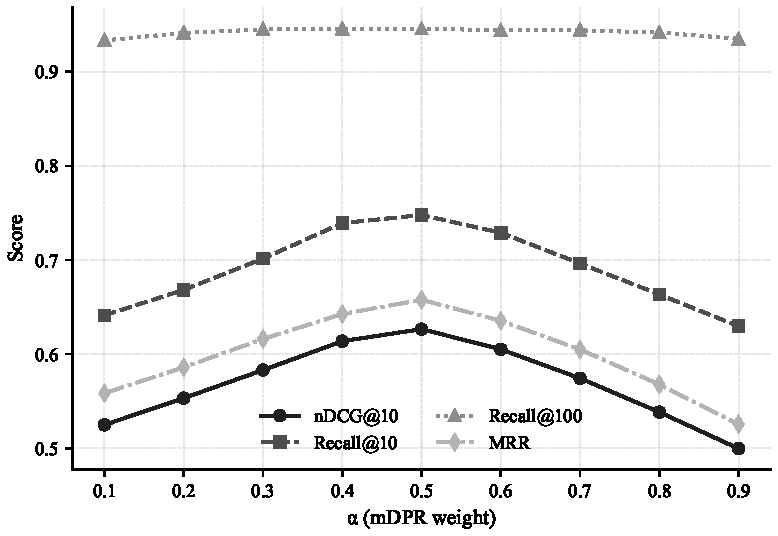
\includegraphics[width=0.95\textwidth]{fig_4_9_alpha_sweep_v2_all.pdf}
  \caption{Convex-combination $\alpha$ sweep for the no-QE hybrid baseline, showing nDCG@10, Recall@\{10,100\} and MRR. nDCG@10 peaks near $\alpha = 0.5$; Recall@100 is largely insensitive to $\alpha$.}
  \label{fig:hybrid_alpha}
\end{figure}

% ─────────────────────────────────────────────────────────────────────
\newpage
\previewheader{Table 4.5}{CSQE component ablation}{§4.8}
\begin{table}[H]
  \centering
  \caption{Ablation of the CSQE pseudo-document, comparing corpus-only, blind-only, and the 2-corpus + 2-blind combination on BM25 alone and within the best hybrid configuration.}
  \label{tab:csqe_ablation}
  \scriptsize
  \begin{tabular}{lcccc}
\toprule
System & nDCG@10 & Recall@10 & Recall@100 & MRR \\
\midrule
BM25 alone (no QE) & 0.462 & 0.596 & 0.858 & 0.484 \\
Hybrid RRF k=20 (no QE) & 0.627 & 0.760 & 0.947 & 0.652 \\
Config A RRF best (Exp 2.1) & 0.714 & 0.836 & 0.973 & 0.736 \\
013d: Blind-only BM25 (0c+4b alpha=4) & 0.575 & 0.709 & 0.920 & 0.603 \\
013c: Corpus-only BM25 (4c+0b alpha=4) & 0.538 & 0.646 & 0.879 & 0.565 \\
013: CSQE BM25 (2c+2b alpha=4) & 0.616 & 0.745 & 0.942 & 0.638 \\
013d + Dense RRF (Config A) & 0.708 & 0.829 & 0.961 & 0.732 \\
013c + Dense RRF (Config A) & 0.662 & 0.790 & 0.951 & 0.681 \\
013 + Dense RRF (Config A) & 0.714 & 0.836 & 0.973 & 0.736 \\
\bottomrule
\end{tabular}

\end{table}

% ─────────────────────────────────────────────────────────────────────
\newpage
\previewheader{Table 4.6}{CSQE vs blind QE on BM25 + Dense}{§4.8}
\begin{table}[H]
  \centering
  \caption{Comparison of CSQE against blind Query2Doc using Aya Expanse 8B as the generator, evaluated on the BM25 and Dense retrievers in isolation.}
  \label{tab:csqe_vs_blind}
  \begin{tabular}{lcc}
\toprule
Variant & BM25 nDCG@10 & Dense nDCG@10 \\
\midrule
No QE (baseline) & 0.4621 & 0.4993 \\
Aya 8B blind QE & 0.5855 & 0.6164 \\
Aya 8B CSQE & 0.6157 & 0.5915 \\
\bottomrule
\end{tabular}

\end{table}

% ─────────────────────────────────────────────────────────────────────
\newpage
\previewheader{Table 4.7}{Configs (BM25-only-expanded / Dense-only-expanded / Both-expanded)}{§4.9}
\begin{table}[H]
  \centering
  \caption{Performance of the three retriever-assignment configurations across CC and RRF fusion, with the no-QE hybrid baseline and BM25/CSQE / Dense/CSQE running alone for reference.}
  \label{tab:configs_abc}
  \scriptsize
  \begin{tabular}{lcccc}
\toprule
Method & nDCG@10 & Recall@10 & Recall@100 & MRR \\
\midrule
BM25 alone & 0.462 & 0.596 & 0.858 & 0.484 \\
mDPR alone & 0.499 & 0.616 & 0.841 & 0.533 \\
Hybrid RRF k=20 (Exp 1.2) & 0.627 & 0.760 & 0.947 & 0.652 \\
BM25+CSQE (Exp 013) & 0.616 & 0.745 & 0.942 & 0.638 \\
Dense+CSQE (Exp 013) & 0.592 & 0.707 & 0.882 & 0.623 \\
BM25-only-expanded CC (alpha=0.6) & 0.709 & 0.830 & 0.972 & 0.727 \\
BM25-only-expanded RRF (k=20) & 0.714 & 0.836 & 0.973 & 0.736 \\
Dense-only-expanded CC (alpha=0.4) & 0.659 & 0.785 & 0.957 & 0.678 \\
Dense-only-expanded RRF (k=20) & 0.647 & 0.793 & 0.957 & 0.658 \\
Both-expanded CC (alpha=0.5) & 0.696 & 0.825 & 0.965 & 0.708 \\
Both-expanded RRF (k=20) & 0.694 & 0.829 & 0.966 & 0.704 \\
\bottomrule
\end{tabular}

\end{table}

% ─────────────────────────────────────────────────────────────────────
\newpage
\previewheader{Figure 4.11 v2}{System progression — \textbf{HEADLINE}}{§4.9}
\begin{figure}[H]
  \centering
  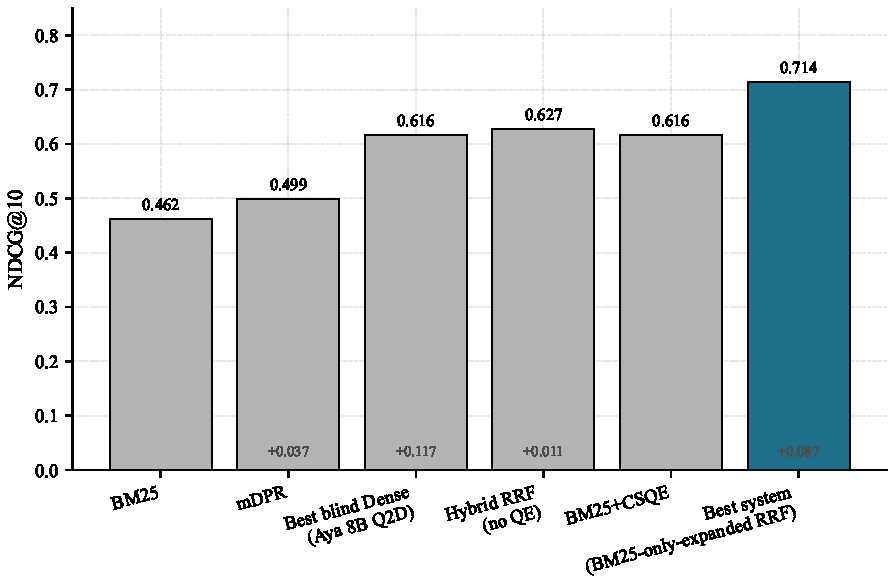
\includegraphics[width=0.95\textwidth]{fig_4_11_progression_v2_annot.pdf}
  \caption{Progression of nDCG@10 from the BM25 baseline (0.462) through intermediate query-enhancement steps to the best system, BM25-only-expanded with RRF fusion, at 0.714. The annotation on each bar reports the gain over the best previous configuration.}
  \label{fig:progression}
\end{figure}

% ─────────────────────────────────────────────────────────────────────
\newpage
\previewheader{Figure 4.12}{Per-query $\Delta$ nDCG@10 — CSQE+Hybrid vs Aya-blind}{§4.10}
\begin{figure}[H]
  \centering
  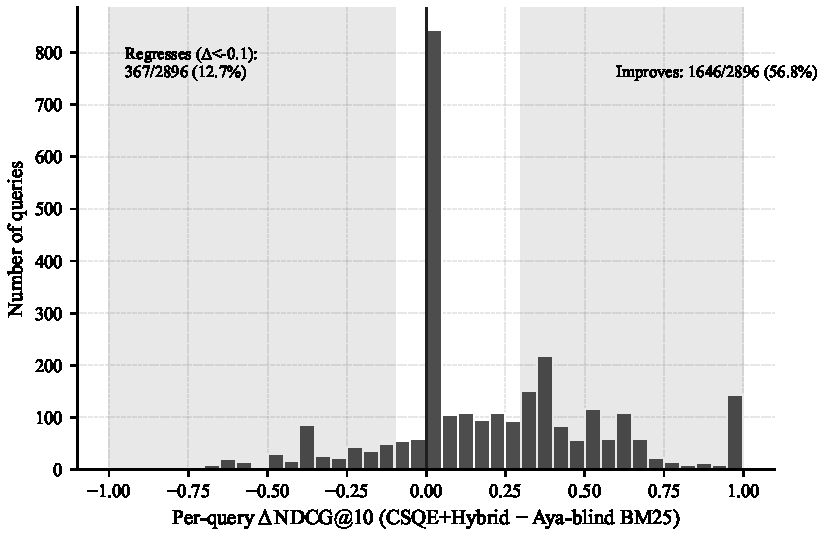
\includegraphics[width=0.85\textwidth]{fig_4_12_delta_hist_v1.pdf}
  \caption{Distribution of the per-query difference between the CSQE+Hybrid system and the Aya-blind BM25 baseline. Shaded bands mark the Big Win region ($\Delta > 0.3$) and the Regression region ($\Delta < -0.1$); 56.8\% of queries improve, 16.6\% regress.}
  \label{fig:delta_dist}
\end{figure}

% ─────────────────────────────────────────────────────────────────────
\newpage
\previewheader{Figure 4.13 v2}{nDCG@10 by first-pass relevance (with sample sizes)}{§4.10}
\begin{figure}[H]
  \centering
  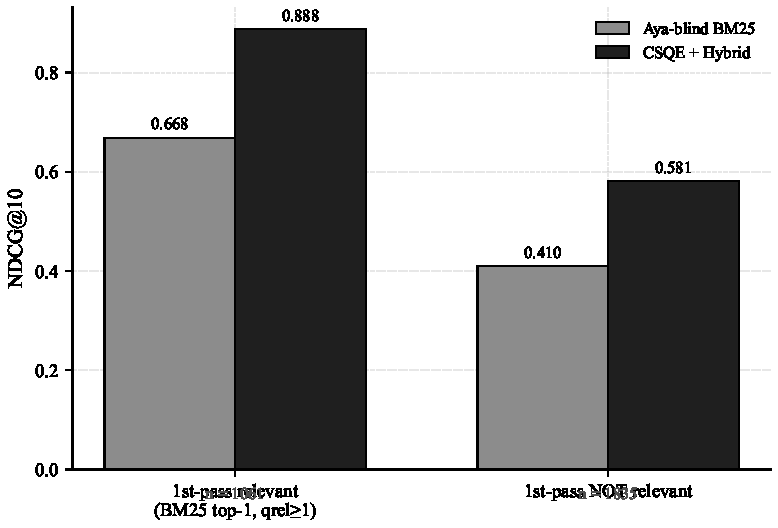
\includegraphics[width=0.85\textwidth]{fig_4_13_firstpass_v2_annot.pdf}
  \caption{CSQE+Hybrid versus Aya-blind baseline conditioned on whether the BM25 first-pass top-1 document is relevant (qrel $\ge$ 1). When the first-pass document is relevant ($n = 1{,}061$) CSQE+Hybrid reaches 0.888 nDCG@10; when it is not ($n = 1{,}835$) it reaches 0.581.}
  \label{fig:first_pass}
\end{figure}

% ─────────────────────────────────────────────────────────────────────
\newpage
\previewheader{Figure 4.14 v2}{$\Delta$ nDCG@10 by query length, grouped blind vs CSQE}{§4.10}
\begin{figure}[H]
  \centering
  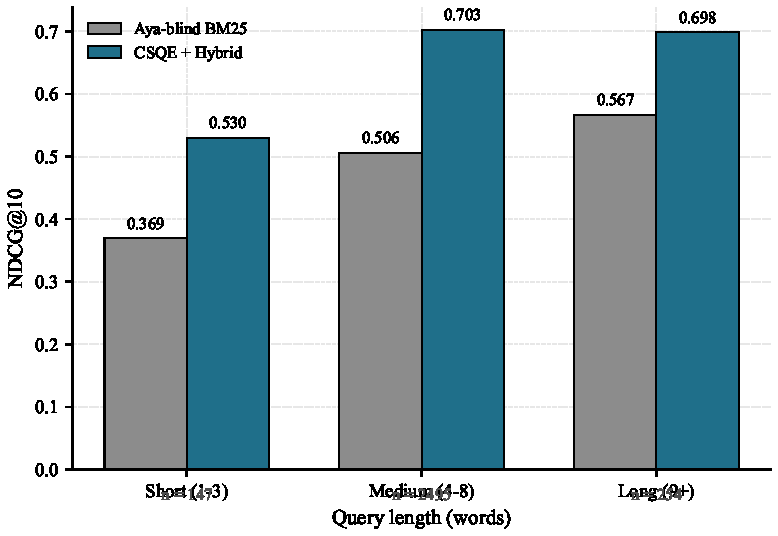
\includegraphics[width=0.85\textwidth]{fig_4_14_lengthgain_v2_grouped.pdf}
  \caption{Per-bucket comparison of Aya-blind BM25 and CSQE+Hybrid using the 1--3 / 4--8 / 9+ word buckets. CSQE+Hybrid improves every bucket; short queries gain the most proportionally (+43.6\%) and medium queries the most absolutely (+0.197).}
  \label{fig:length_gain}
\end{figure}

% ─────────────────────────────────────────────────────────────────────
\newpage
\previewheader{Figure 4.15 v2}{Regression types breakdown (donut, $n = 367$)}{§4.10}
\begin{figure}[H]
  \centering
  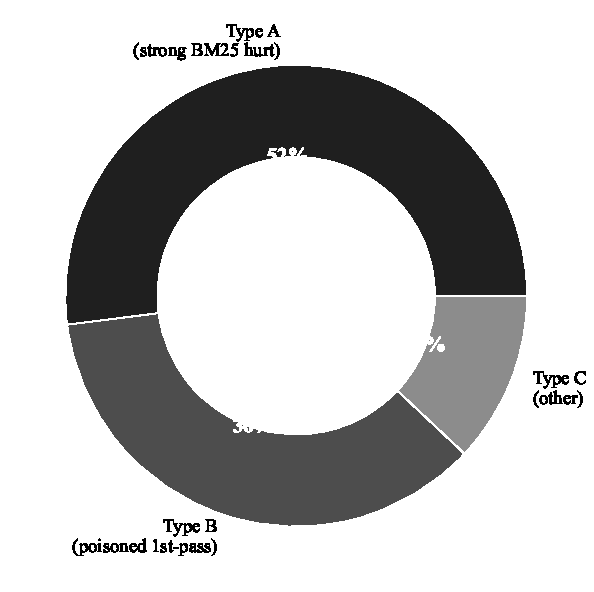
\includegraphics[width=0.6\textwidth]{fig_4_15_regtype_v2_donut.pdf}
  \caption{Type breakdown of the 367 queries that regress under CSQE+Hybrid ($\Delta < -0.1$). Type A (strong-BM25-hurt-by-expansion) accounts for 52\%, Type B (poisoned first-pass) for 36\%, and Type C (other) for 12\%.}
  \label{fig:regression_types}
\end{figure}

\end{document}
